\documentclass[tikz,border=0pt]{standalone}
\usepackage[american]{circuitikz}
\usetikzlibrary{arrows.meta,calc,positioning,decorations.pathmorphing,patterns}
\definecolor{zyloTeal}{HTML}{174A5B}
\definecolor{zyloTealTwo}{HTML}{246B7A}
\definecolor{zyloInk}{HTML}{1F2933}
\definecolor{zyloSoft}{HTML}{EAF4F4}
\definecolor{zyloPaper}{HTML}{F8FAFB}
\definecolor{zyloLine}{HTML}{44606B}
\definecolor{zyloOrange}{HTML}{D97706}
\begin{document}
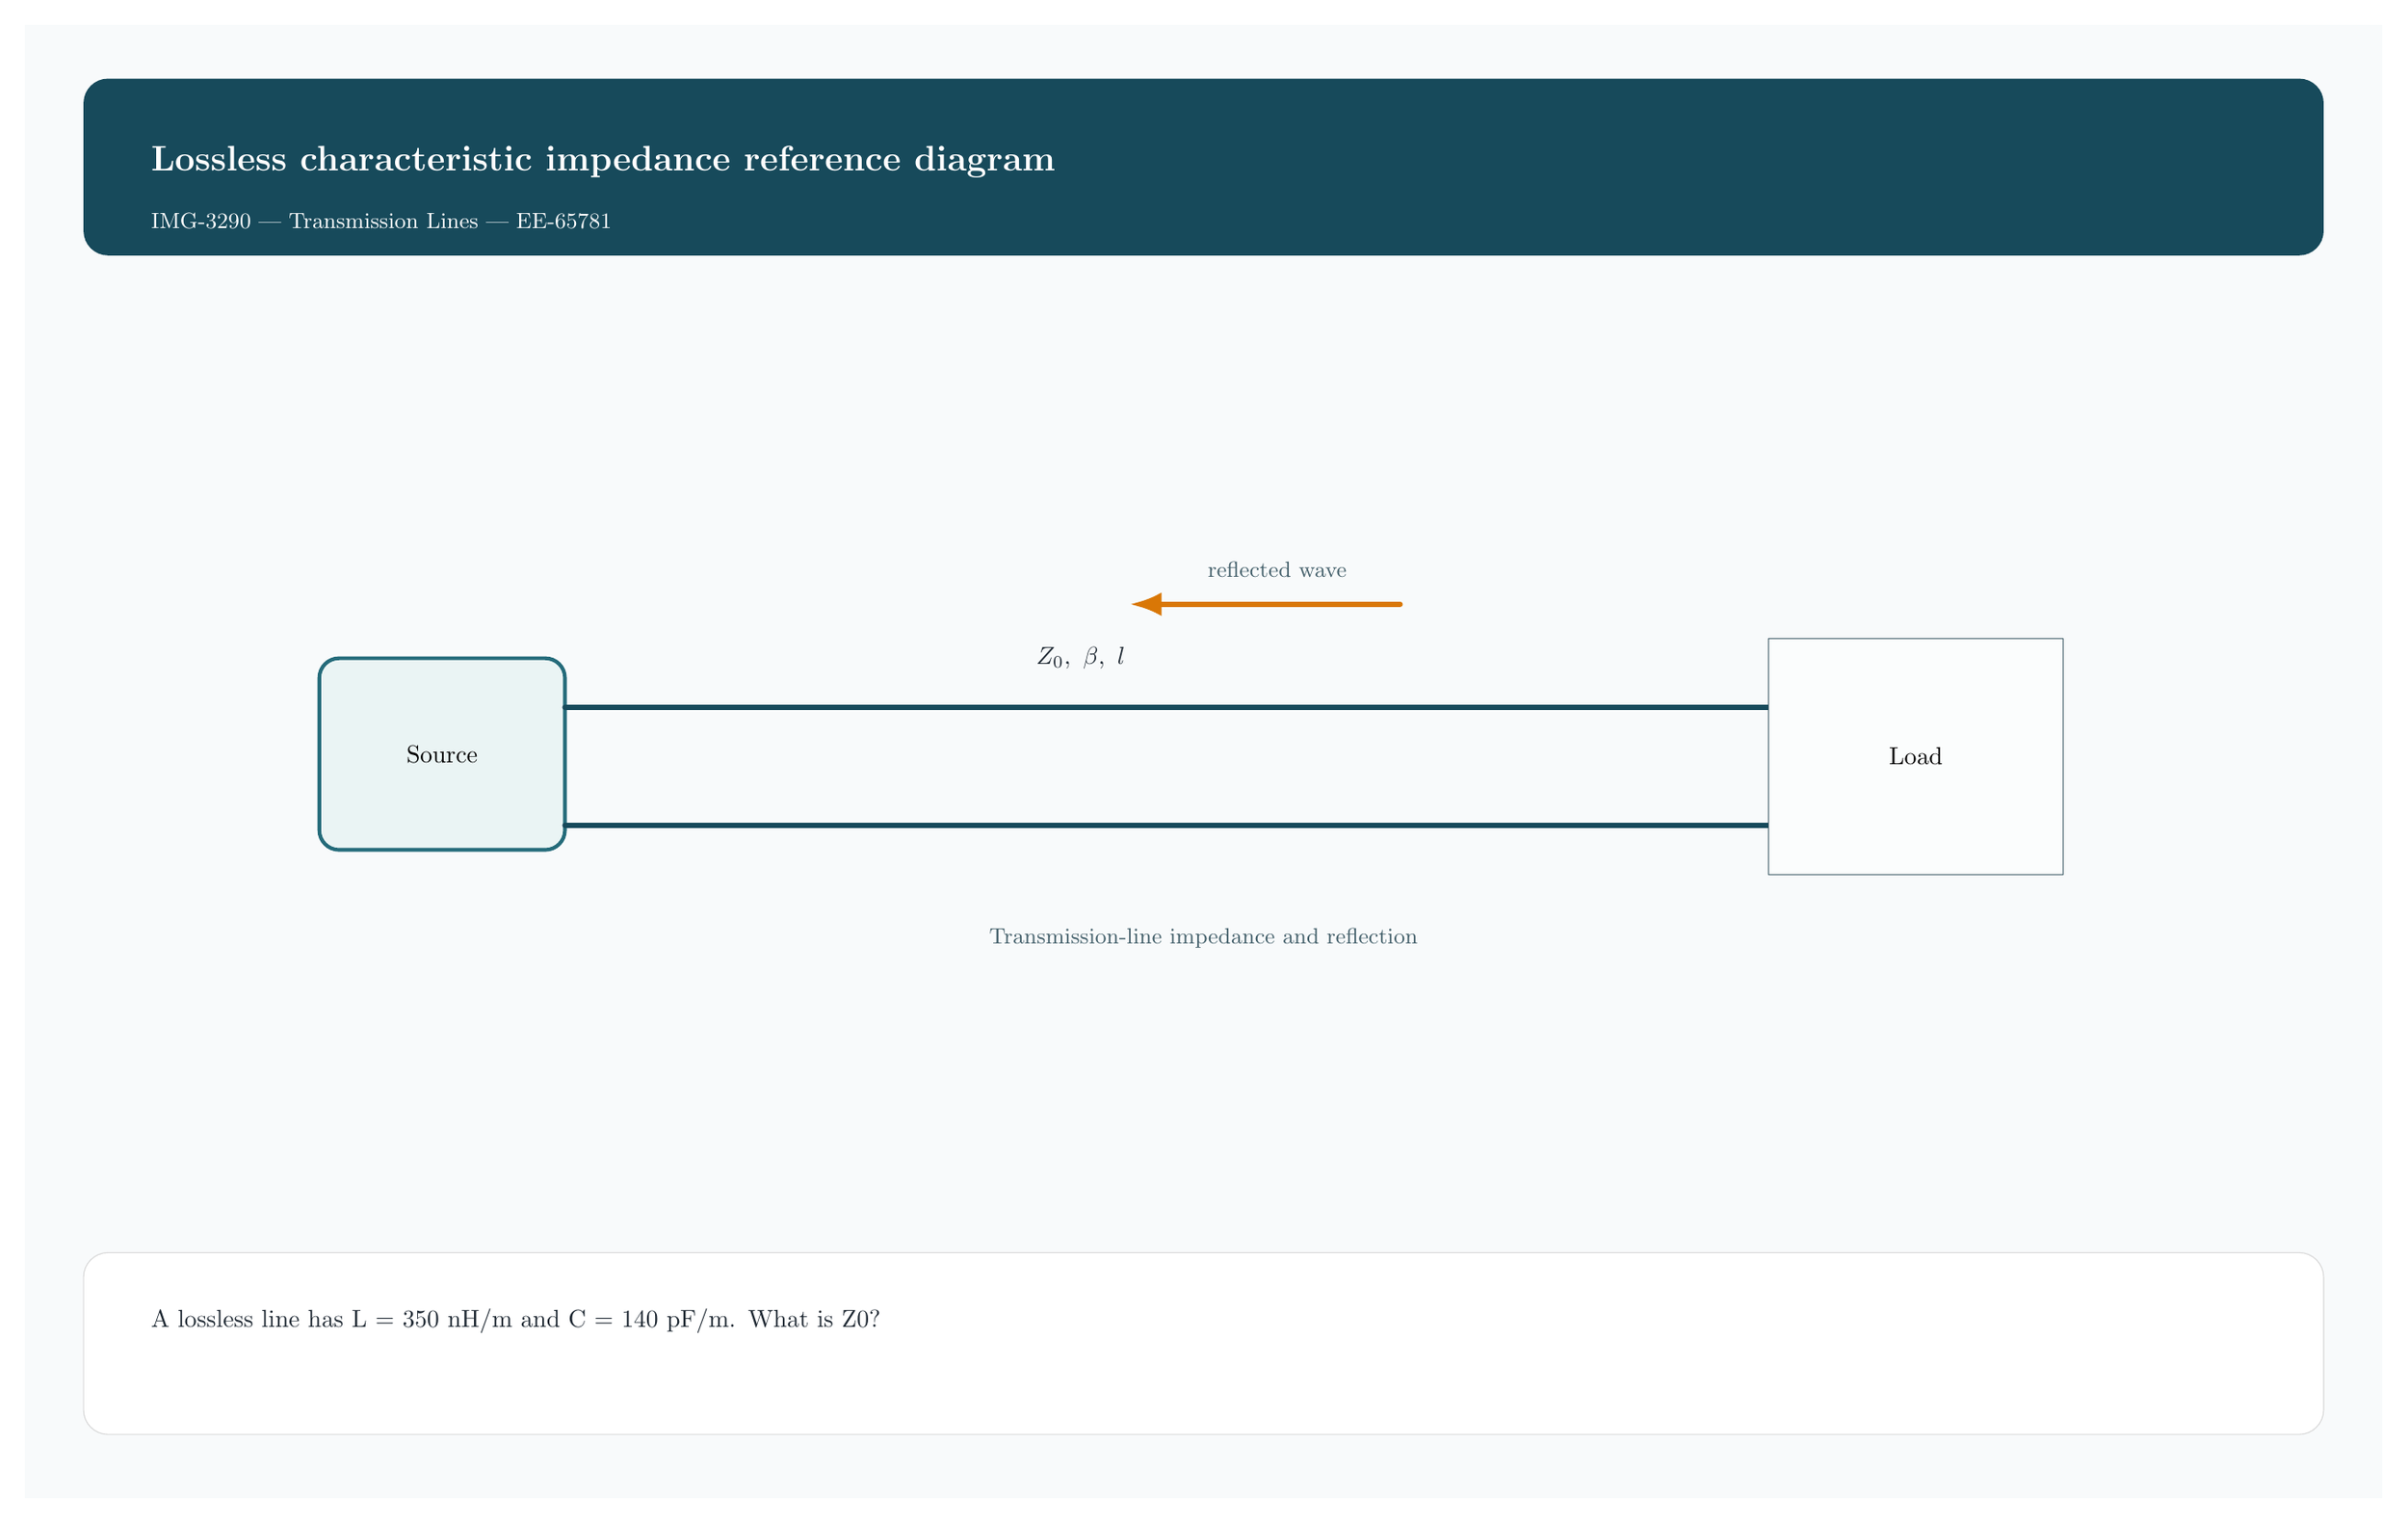
\begin{tikzpicture}[x=1pt,y=-1pt,>=Latex,line cap=round,line join=round]
\path[fill=zyloPaper] (0,0) rectangle (960,600);
\path[fill=zyloTeal,rounded corners=10pt] (24,22) rectangle (936,94);
\node[anchor=west,text=white,font=\bfseries\Large] at (48,56) {Lossless characteristic impedance reference diagram};
\node[anchor=west,text=white!82,font=\small] at (48,80) {IMG-3290 | Transmission Lines | EE-65781};
\tikzset{wire/.style={draw=zyloTeal,line width=2.2pt},thinwire/.style={draw=zyloLine,line width=1.35pt},accent/.style={draw=zyloOrange,line width=2.2pt},box/.style={draw=zyloTealTwo,fill=zyloSoft,line width=1.5pt,rounded corners=8pt}}
\node[box,minimum width=100pt,minimum height=78pt] at (170,297) {Source};
\draw[wire] (220,278) -- (710,278);
\draw[wire] (220,326) -- (710,326);
\node[draw=zyloLine,fill=white!80!zyloSoft,minimum width=120pt,minimum height=96pt] at (770,298) {Load};
\node[text=zyloInk] at (430,258) {$Z_0,\ \beta,\ l$};
\draw[accent,->] (560,236) -- (450,236); \node[font=\small,text=zyloLine] at (510,222) {reflected wave};
\node[font=\small,text=zyloLine] at (480,372) {Transmission-line impedance and reflection};
\path[draw=black!15,fill=white,rounded corners=10pt] (24,500) rectangle (936,574);
\node[anchor=west,text width=860pt,align=left,text=zyloInk,font=\normalsize] at (48,528) {A lossless line has L = 350 nH/m and C = 140 pF/m. What is Z0?};
\end{tikzpicture}
\end{document}
